\documentclass[UTF8,fontset=fandol,aspectratio=169,10pt]{ctexbeamer}
\usepackage{booktabs,array,graphicx,tikz,amsmath}
\usetikzlibrary{positioning,arrows.meta}
\definecolor{navy}{HTML}{20364C}\definecolor{teal}{HTML}{147D92}
\setbeamercolor{normal text}{fg=navy,bg=white}
\setbeamercolor{structure}{fg=teal}
\setbeamercolor{frametitle}{fg=navy,bg=white}
\setbeamerfont{frametitle}{size=\large,series=\bfseries}
\setbeamertemplate{navigation symbols}{}
\setbeamertemplate{footline}{\hfill\color{gray}\scriptsize\insertframenumber\hspace{0.5cm}\vspace{0.2cm}}
\setbeamersize{text margin left=0.7cm,text margin right=0.7cm}
\setbeamertemplate{itemize item}{\color{teal}\small$\bullet$}
\setlength{\parskip}{5pt}\emergencystretch=2em
\begin{document}
\begin{frame}{PyTorch/\allowbreak{}CUDA 可达域工程}
\vspace{0.5cm}{\LARGE 阶段进展与实验对照}\par\vspace{0.6cm}
{\large 做了什么，哪些任务更快，范围差距在哪里}\par\vspace{0.8cm}
我们 / Huan / Xiangru / Native Flow*\par
\vspace{0.3cm}2026年9月23日\par
\vfill\color{teal}本次资料整理和新分支推送完成后暂停工作
\end{frame}
\begin{frame}{当前进展}
\begin{itemize}
\item 完整 GPU 引擎已跑通：四个固定多项式任务有完整时间与宽度对照。
\item TORA 新候选从部分失败改善到 2400/\allowbreak{}2400 分区步成功。
\item 范围输出取得 15.3\%–43.6\% 的五次配对耗时下降。
\item 主要缺口：原式 VDP 单盒仍慢且略宽；TORA 后段明显偏宽；控制器严格误差资格未完成。
\end{itemize}\par\vfill{\fontsize{6.5}{8}\selectfont\color{gray}证据：S1–S5、S7；各项使用不同且明确分开的实验口径。} 
\end{frame}
\begin{frame}{可达域计算的目标}
\begin{columns}[T]
\begin{column}{0.55\textwidth}
给定方程、初始状态集合和时间：
\begin{itemize}
\item 包住所有可能轨迹
\item 范围越紧，安全判断越有用
\item 算得快，也要保持误差覆盖
\end{itemize}
\vspace{0.3cm}普通模拟只回答“这一条轨迹怎么走”；这里计算整个集合的包络。
\end{column}
\begin{column}{0.40\textwidth}
\begin{tikzpicture}[x=0.54cm,y=0.54cm]
\draw[->,gray] (0,0)--(7.5,0) node[right]{时间};
\draw[->,gray] (0,0)--(0,5.3) node[above]{状态};
\fill[teal!15] (0,1.3) .. controls (2,1.4) and (4,2.3) .. (7,2.6) -- (7,4.6) .. controls (4,4.0) and (2,3.3) .. (0,2.7) -- cycle;
\draw[teal,thick] (0,1.3) .. controls (2,1.4) and (4,2.3) .. (7,2.6);
\draw[teal,thick] (0,2.7) .. controls (2,3.3) and (4,4.0) .. (7,4.6);
\draw[navy] (0,2) .. controls (2,2.1) and (4,3.5) .. (7,3.7);
\node[teal] at (4.3,4.9) {集合包络示意};
\end{tikzpicture}
\end{column}\end{columns}
\end{frame}
\begin{frame}{完整计算链}
\begin{center}
\begin{tikzpicture}[node distance=0.7cm, every node/.style={align=center}]
\node[draw=teal,fill=teal!7,text width=2.6cm,minimum height=1.2cm] (a) {初始状态盒\\与系统方程};
\node[draw=teal,fill=teal!7,text width=2.8cm,minimum height=1.2cm,right=of a] (b) {Taylor model 推进\\多项式 + 区间余项};
\node[draw=teal,fill=teal!7,text width=2.6cm,minimum height=1.2cm,right=of b] (c) {验证与 SR 历史\\成功才提交};
\node[draw=teal,fill=teal!7,text width=2.3cm,minimum height=1.2cm,right=of c] (d) {物理范围\\endpoint / tube};
\draw[->,thick,teal] (a)--(b);\draw[->,thick,teal] (b)--(c);\draw[->,thick,teal] (c)--(d);
\end{tikzpicture}\end{center}
\vspace{0.4cm}
\begin{itemize}
\item Taylor model 保留状态依赖；余项承担截断及浮点误差
\item SR 保留跨步误差关系，减轻反复装箱导致的膨胀
\item 本阶段优化完整推进和范围输出，失败仍按原规则回滚
\end{itemize}
\end{frame}
\begin{frame}{三个仓库与四类实现}
{\fontsize{8.5}{11}\selectfont
{\setlength{\tabcolsep}{2pt}\renewcommand{\arraystretch}{1.25}
\begin{tabular}{>{\raggedright\arraybackslash}p{0.331\linewidth}>{\raggedright\arraybackslash}p{0.340\linewidth}>{\raggedright\arraybackslash}p{0.248\linewidth}}
\toprule
\textbf{角色} & \textbf{使用内容} & \textbf{比较版本} \\
\midrule
我们：torch\_\allowbreak{}tm\_\allowbreak{}flowpipe & 工程、适配与严格优化 & plant f536；NNCS fff9 \\
Huan：flowstar-gpu & 原始GPU引擎及证明背景 & d5f0b68f \\
Xiangru：CROWN-Reach & 集成驱动、模型、benchmark & 1c16d4ef \\
Native Flow* & C++可达域参考 & 固定匹配构建 \\
\bottomrule
\end{tabular}
}
}\par
\begin{itemize}
\item 我们复用已有引擎和修复；主比较是具体版本的完整实现差异。
\item NNCS 中 Huan/\allowbreak{}Xiangru 分别接入同一个 Xiangru 驱动。
\end{itemize}\par\vfill{\fontsize{6.5}{8}\selectfont\color{gray}详细仓库URL、完整源码/\allowbreak{}库身份：REPORT.md 第3节与 configs/\allowbreak{}plant\_\allowbreak{}contracts.json。} 
\end{frame}
\begin{frame}{主要改动}
{\fontsize{8.5}{11}\selectfont
{\setlength{\tabcolsep}{2pt}\renewcommand{\arraystretch}{1.25}
\begin{tabular}{>{\raggedright\arraybackslash}p{0.175\linewidth}>{\raggedright\arraybackslash}p{0.460\linewidth}>{\raggedright\arraybackslash}p{0.285\linewidth}}
\toprule
\textbf{方向} & \textbf{做了什么} & \textbf{希望改善什么} \\
\midrule
完整GPU执行 & 稀疏/\allowbreak{}Horner计算、CUDA图、SR准备复用 & 减少完整任务调度与组织成本 \\
数值表示 & 线性路径保留更多多项式信息，沿原积分验证承载误差 & 减少不必要的余项膨胀与拒绝 \\
范围输出 & 保留向外舍入次序，原生CPU乘法加快展开 & 让用户真正拿到范围的过程更快 \\
相同实验 & 固定配置、完整轨迹、五次计时、所有失败记录 & 让时间和宽度的比较可信 \\
\bottomrule
\end{tabular}
}
}\par

\end{frame}
\begin{frame}{时间与宽度如何读取}
{\fontsize{8.5}{11}\selectfont
{\setlength{\tabcolsep}{2pt}\renewcommand{\arraystretch}{1.25}
\begin{tabular}{>{\raggedright\arraybackslash}p{0.184\linewidth}>{\raggedright\arraybackslash}p{0.350\linewidth}>{\raggedright\arraybackslash}p{0.386\linewidth}}
\toprule
\textbf{数字} & \textbf{含义} & \textbf{容易误读的地方} \\
\midrule
核心秒数 & 完整推进含初始化、图捕获、SR和同步 & 不含进程启动和独立输出 \\
进程秒数 & runner启动到退出 & 含控制器等启动；仍不含独立导出 \\
宽度比 & 当前范围宽度 /\allowbreak{} Flow*范围宽度 & 1接近；更小不是正确性证明 \\
p95 /\allowbreak{} max & 逐通道统计，再取最差通道 & 不能删最差步或只报中位 \\
成功分区步 & 全部真实分区的接受步数 & 不完整任务不能作成功加速分母 \\
\bottomrule
\end{tabular}
}
}\par
\par\vfill{\fontsize{6.5}{8}\selectfont\color{gray}Endpoint：步末范围；tube：整步范围。报告附录保留两类输出和每一物理坐标。} 
\end{frame}
\begin{frame}{固定多项式实验配置}
{\fontsize{8.5}{11}\selectfont
{\setlength{\tabcolsep}{2pt}\renewcommand{\arraystretch}{1.25}
\begin{tabular}{>{\raggedright\arraybackslash}p{0.230\linewidth}>{\raggedright\arraybackslash}p{0.345\linewidth}>{\raggedright\arraybackslash}p{0.345\linewidth}}
\toprule
\textbf{参数} & \textbf{Van der Pol} & \textbf{Brusselator} \\
\midrule
原盒 & [1.1,1.4] × [2.35,2.45] & [1.48,1.52] × [2.98,3.02] \\
阶数 /\allowbreak{} h & 4 /\allowbreak{} 0.01 & 6 /\allowbreak{} 0.02 \\
完整单盒 & B1×1000，T10 & B1×1000，T20 \\
真实分区 & 8×4，B32×20，T0.2 & 8×4，B32×20，T0.4 \\
cutoff /\allowbreak{} 余项半径 & 1e−10 /\allowbreak{} 1e−4 & 1e−10 /\allowbreak{} 1e−4 \\
SR容量 & 100 & 1000 \\
\bottomrule
\end{tabular}
}
}\par
V100 16GB /\allowbreak{} Xeon Gold 6138；单CPU线程；每组五次；共120次。\par
\par\vfill{\fontsize{6.5}{8}\selectfont\color{gray}S1/\allowbreak{}S6。VDP 主比较固定原式 y−x−x*x*y；分区不是复制同一盒。} 
\end{frame}
\begin{frame}{固定任务：完整核心时间}
\begin{center}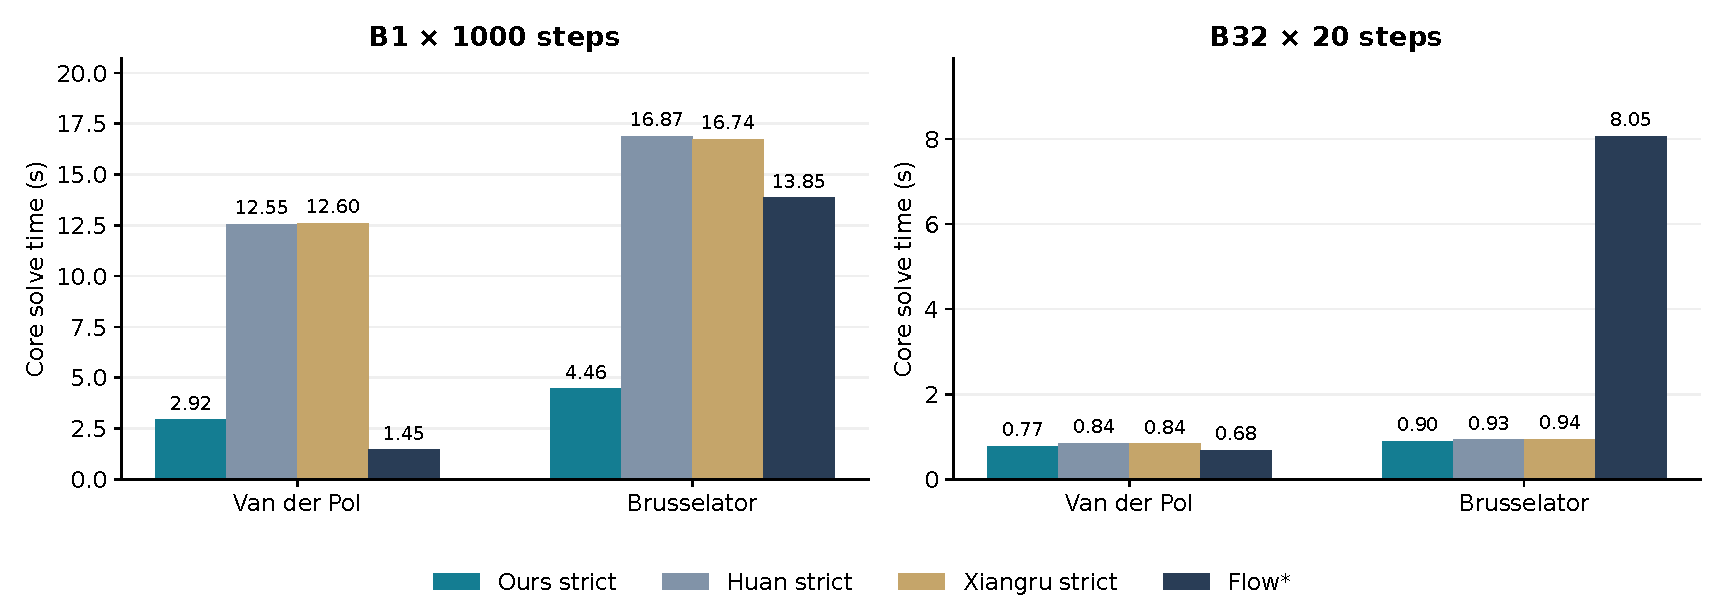
\includegraphics[width=\linewidth,height=5.45cm,keepaspectratio]{figures/plant_core.pdf}\end{center}B1 显著快于原版 strict；VDP B1 仍慢于 Flow*。\par
\par\vfill{\fontsize{6.5}{8}\selectfont\color{gray}S1：五次中位秒，全部完成。初始化/\allowbreak{}捕获计入；进程启动与输出排除。} 
\end{frame}
\begin{frame}{固定任务：具体时间与达标情况}
{\fontsize{8.5}{11}\selectfont
{\setlength{\tabcolsep}{2pt}\renewcommand{\arraystretch}{1.25}
\begin{tabular}{>{\raggedright\arraybackslash}p{0.239\linewidth}>{\raggedright\arraybackslash}p{0.170\linewidth}>{\raggedright\arraybackslash}p{0.170\linewidth}>{\raggedright\arraybackslash}p{0.170\linewidth}>{\raggedright\arraybackslash}p{0.170\linewidth}}
\toprule
\textbf{任务} & \textbf{我们} & \textbf{Huan} & \textbf{Xiangru} & \textbf{Flow*} \\
\midrule
Van der Pol B1 & 2.921487 & 12.552073 & 12.602979 & 1.447977 \\
Van der Pol B32 & 0.769654 & 0.840225 & 0.837461 & 0.682880 \\
Brusselator B1 & 4.456490 & 16.867330 & 16.737087 & 13.847315 \\
Brusselator B32 & 0.897973 & 0.929344 & 0.935446 & 8.053289 \\
\bottomrule
\end{tabular}
}
}\par
单位：核心秒，五次中位数；三种 GPU 实现均为 strict。\par
\vspace{0.25cm}{\fontsize{8.5}{11}\selectfont
{\setlength{\tabcolsep}{2pt}\renewcommand{\arraystretch}{1.25}
\begin{tabular}{>{\raggedright\arraybackslash}p{0.258\linewidth}>{\raggedright\arraybackslash}p{0.166\linewidth}>{\raggedright\arraybackslash}p{0.166\linewidth}>{\raggedright\arraybackslash}p{0.166\linewidth}>{\raggedright\arraybackslash}p{0.166\linewidth}}
\toprule
\textbf{我们 /\allowbreak{} Flow* 配对比} & \textbf{VDP B1} & \textbf{VDP B32} & \textbf{Bruss B1} & \textbf{Bruss B32} \\
\midrule
目标 $\leq$1.20 & 2.015 未达 & 1.129 达到 & 0.322 达到 & 0.111 达到 \\
\bottomrule
\end{tabular}
}
}\par
\par\vfill{\fontsize{6.5}{8}\selectfont\color{gray}S1；比值来自同轮配对，中位数之比不作为配对比替代。} 
\end{frame}
\begin{frame}{固定任务：具体全程宽度}
{\fontsize{8.5}{11}\selectfont
{\setlength{\tabcolsep}{2pt}\renewcommand{\arraystretch}{1.25}
\begin{tabular}{>{\raggedright\arraybackslash}p{0.230\linewidth}>{\raggedright\arraybackslash}p{0.230\linewidth}>{\raggedright\arraybackslash}p{0.230\linewidth}>{\raggedright\arraybackslash}p{0.230\linewidth}}
\toprule
\textbf{任务} & \textbf{我们 strict} & \textbf{Huan strict} & \textbf{Xiangru strict} \\
\midrule
Van der Pol B1 & 1.123238 /\allowbreak{} 1.271071 & 1.297229 /\allowbreak{} 1.718783 & 1.297229 /\allowbreak{} 1.718783 \\
Van der Pol B32 & 1.000597 /\allowbreak{} 1.000656 & 1.000040 /\allowbreak{} 1.000047 & 1.000040 /\allowbreak{} 1.000047 \\
Brusselator B1 & 1.012228 /\allowbreak{} 1.038326 & 1.641986 /\allowbreak{} 4.291133 & 1.641986 /\allowbreak{} 4.291133 \\
Brusselator B32 & 1.000400 /\allowbreak{} 1.000442 & 1.000007 /\allowbreak{} 1.000010 & 1.000007 /\allowbreak{} 1.000010 \\
\bottomrule
\end{tabular}
}
}\par
\vspace{0.35cm}\begin{itemize}
\item 每格：最差通道 p95 /\allowbreak{} max；Flow* 自身为 1 /\allowbreak{} 1。
\item 目标：p95 $\leq$1.10，max $\leq$1.25；原式 VDP B1 仍未达到。
\item 其余三项达到；B1 长轨迹比作者 strict 更接近 Flow*。
\end{itemize}\par\vfill{\fontsize{6.5}{8}\selectfont\color{gray}S2：65,600行、80通道；全部真实分区与全轨迹。} 
\end{frame}
\begin{frame}{VDP：范围差距出现在后段}
\begin{center}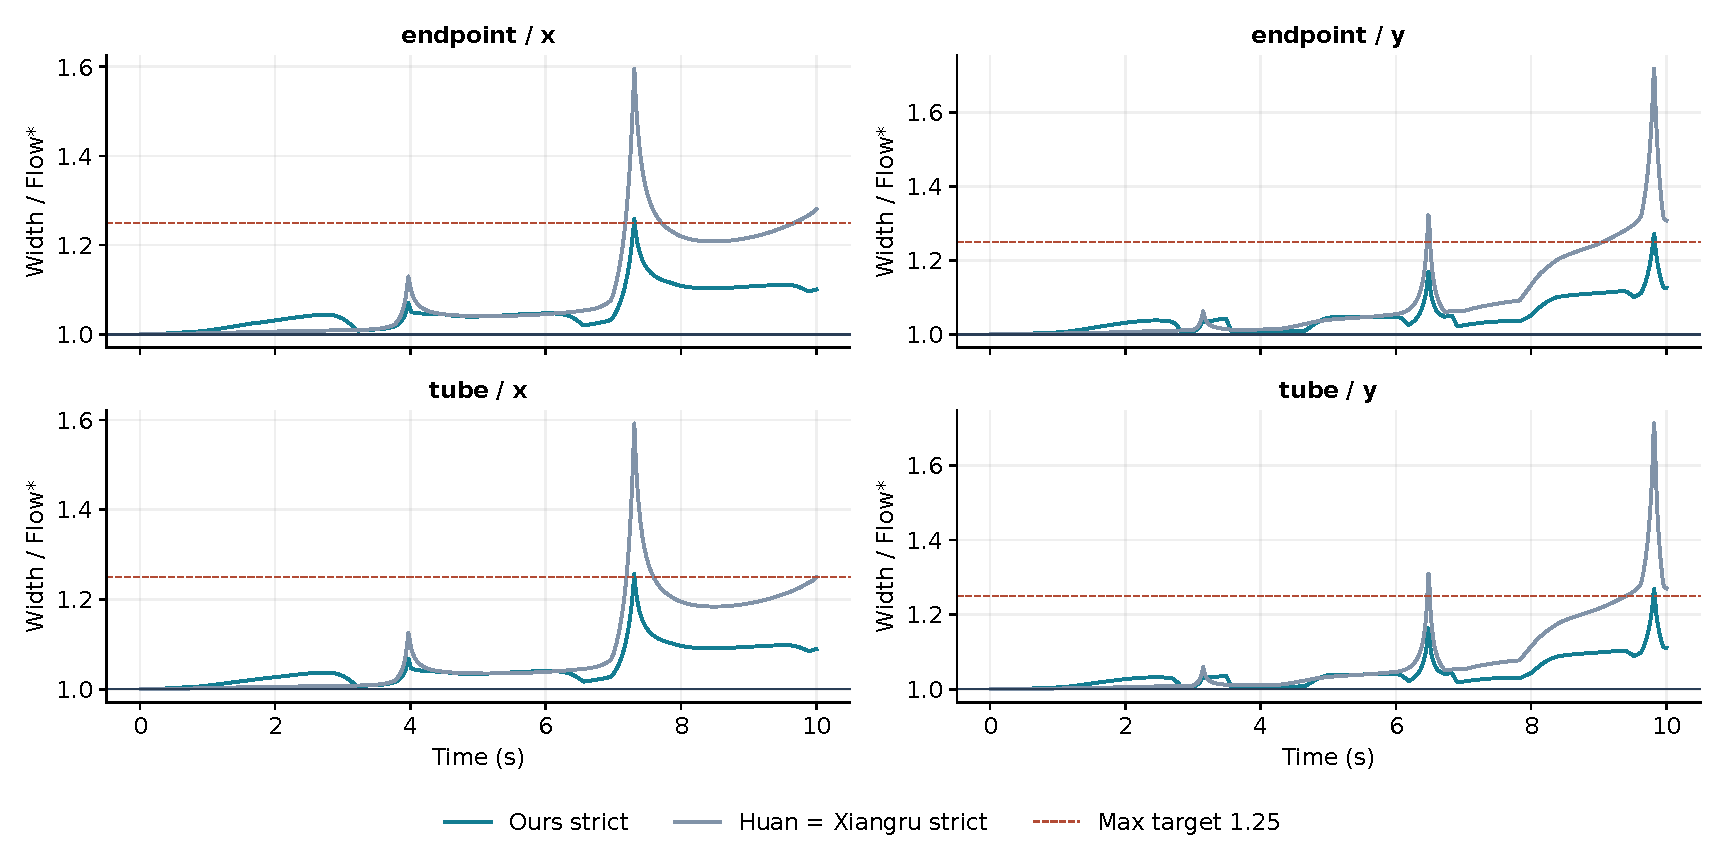
\includegraphics[width=\linewidth,height=6cm,keepaspectratio]{figures/van_der_pol_widths.pdf}\end{center}\par\vfill{\fontsize{6.5}{8}\selectfont\color{gray}原式 B1×1000；分开展示 endpoint/\allowbreak{}tube 与 x/\allowbreak{}y；虚线为最大值门槛1.25。} 
\end{frame}
\begin{frame}{Brusselator：长轨迹范围明显改善}
\begin{center}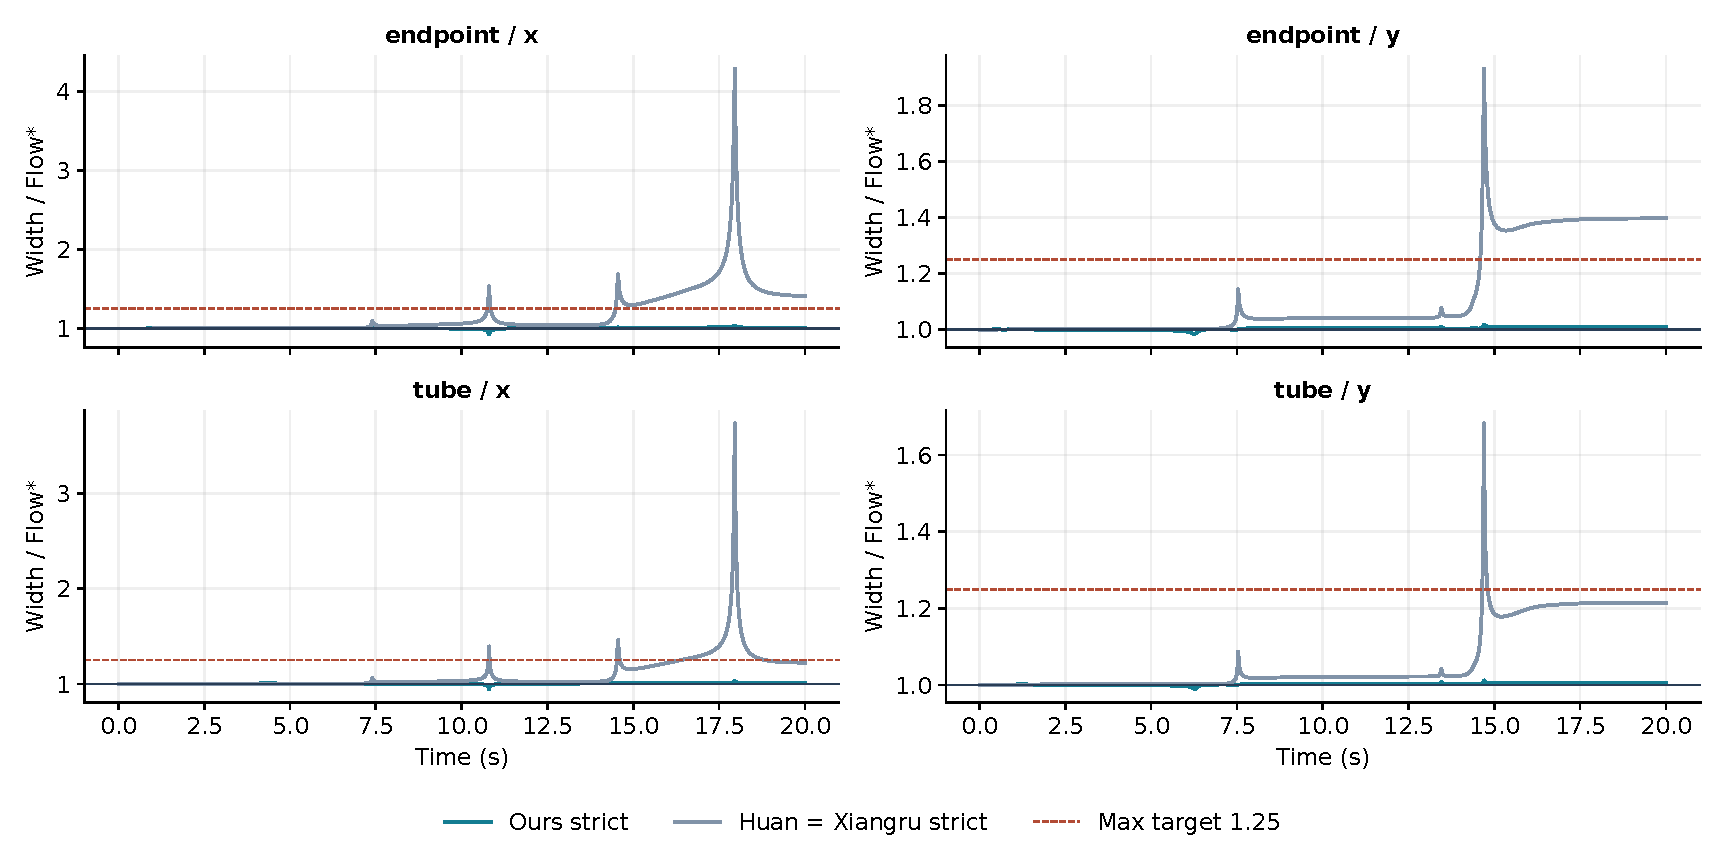
\includegraphics[width=\linewidth,height=6cm,keepaspectratio]{figures/brusselator_widths.pdf}\end{center}\par\vfill{\fontsize{6.5}{8}\selectfont\color{gray}B1×1000；我们最差 p95/\allowbreak{}max=1.012228/\allowbreak{}1.038326。} 
\end{frame}
\begin{frame}{作者闭环控制实验配置}
{\fontsize{8.5}{11}\selectfont
{\setlength{\tabcolsep}{2pt}\renewcommand{\arraystretch}{1.25}
\begin{tabular}{>{\raggedright\arraybackslash}p{0.285\linewidth}>{\raggedright\arraybackslash}p{0.212\linewidth}>{\raggedright\arraybackslash}p{0.212\linewidth}>{\raggedright\arraybackslash}p{0.212\linewidth}}
\toprule
\textbf{参数} & \textbf{TORA} & \textbf{单摆} & \textbf{CartPole} \\
\midrule
B×ODE步数 & 12×200 & 1×100 & 1×200 \\
阶数 /\allowbreak{} h & 3 /\allowbreak{} 0.1 & 2 /\allowbreak{} 0.01 & 6 /\allowbreak{} 0.005 \\
控制周期 × 周期数 & 1.0 × 20 & 0.05 × 20 & 0.02 × 50 \\
总时长 & 20 & 1 & 1 \\
余项猜测 & ±0.01 & ±0.01 & ±0.1 \\
\bottomrule
\end{tabular}
}
}\par
\begin{itemize}
\item 同模型、box /\allowbreak{} same-slope /\allowbreak{} flat /\allowbreak{} rpc-float32 控制合同。
\item 匹配 native 固定步数和共同 binary64 初盒；原始支路另存。
\item TORA/\allowbreak{}单摆各六组五次；CartPole 六组单次完整尝试。
\end{itemize}\par\vfill{\fontsize{6.5}{8}\selectfont\color{gray}S3/\allowbreak{}S4/\allowbreak{}S6。模型、全部初盒、方程与约束在附录和 YAML。} 
\end{frame}
\begin{frame}{TORA：全程成功，进程更快，范围仍宽}
{\fontsize{8.5}{11}\selectfont
{\setlength{\tabcolsep}{2pt}\renewcommand{\arraystretch}{1.25}
\begin{tabular}{>{\raggedright\arraybackslash}p{0.258\linewidth}>{\raggedright\arraybackslash}p{0.147\linewidth}>{\raggedright\arraybackslash}p{0.193\linewidth}>{\raggedright\arraybackslash}p{0.322\linewidth}}
\toprule
\textbf{实现} & \textbf{进程秒} & \textbf{接受分区步} & \textbf{全程p95 /\allowbreak{} max} \\
\midrule
我们 strict v2 & 6.765 & 2400/\allowbreak{}2400 & 1.592229 /\allowbreak{} 2.710606 \\
Huan strict & 7.767 & 2357/\allowbreak{}2400 & 未完整 \\
Xiangru strict & 7.704 & 2357/\allowbreak{}2400 & 未完整 \\
Flow* & 12.238 & 2400/\allowbreak{}2400 & 1.000000 /\allowbreak{} 1.000000 \\
Huan parity & 7.615 & 2400/\allowbreak{}2400 & 1.000000 /\allowbreak{} 1.000000 \\
Xiangru parity & 7.664 & 2400/\allowbreak{}2400 & 1.000000 /\allowbreak{} 1.000000 \\
\bottomrule
\end{tabular}
}
}\par
\vspace{0.25cm}Flow* 耗时 /\allowbreak{} 我们耗时：完整成功进程配对比为 1.802。\par
Huan/\allowbreak{}Xiangru strict 未完整；parity 只作参考，不替代严格保证。\par
\par\vfill{\fontsize{6.5}{8}\selectfont\color{gray}S3/\allowbreak{}S7；五次进程中位秒，含启动及控制器；范围来自独立完整轨迹。} 
\end{frame}
\begin{frame}{TORA：主要数值进展}
{\fontsize{8.5}{11}\selectfont
{\setlength{\tabcolsep}{2pt}\renewcommand{\arraystretch}{1.25}
\begin{tabular}{>{\raggedright\arraybackslash}p{0.350\linewidth}>{\raggedright\arraybackslash}p{0.313\linewidth}>{\raggedright\arraybackslash}p{0.258\linewidth}}
\toprule
\textbf{阶段} & \textbf{成功分区步} & \textbf{首个失败步} \\
\midrule
初始严格版 & 2354 /\allowbreak{} 2400 & 189 \\
直接变量候选 & 2393 /\allowbreak{} 2400 & 197 \\
线性路径 v2 & 2400 /\allowbreak{} 2400 & 全程完成 \\
\bottomrule
\end{tabular}
}
}\par
\vspace{0.3cm}\begin{itemize}
\item 改进多项式信息的保留方式，未改步长、阶数、初盒或控制器。
\item 共同前188步 p95/\allowbreak{}max：2.556/\allowbreak{}8.855 → 1.384/\allowbreak{}1.884。
\item 新v2全程仍为1.592/\allowbreak{}2.711；完成率问题解决，紧度问题仍在。
\end{itemize}\par\vfill{\fontsize{6.5}{8}\selectfont\color{gray}S7；仅加、减、取负的安全线性路径适用；非线性消费者回退。} 
\end{frame}
\begin{frame}{单摆：范围接近，完整进程略慢于 Flow*}
{\fontsize{8.5}{11}\selectfont
{\setlength{\tabcolsep}{2pt}\renewcommand{\arraystretch}{1.25}
\begin{tabular}{>{\raggedright\arraybackslash}p{0.258\linewidth}>{\raggedright\arraybackslash}p{0.147\linewidth}>{\raggedright\arraybackslash}p{0.166\linewidth}>{\raggedright\arraybackslash}p{0.350\linewidth}}
\toprule
\textbf{实现} & \textbf{进程秒} & \textbf{成功步} & \textbf{全程p95 /\allowbreak{} max} \\
\midrule
我们 strict v2 & 5.266 & 100/\allowbreak{}100 & 1.036731 /\allowbreak{} 1.040936 \\
Huan strict & 5.615 & 100/\allowbreak{}100 & 1.067393 /\allowbreak{} 1.075450 \\
Xiangru strict & 5.610 & 100/\allowbreak{}100 & 1.067393 /\allowbreak{} 1.075450 \\
Flow* & 4.987 & 100/\allowbreak{}100 & 1.000000 /\allowbreak{} 1.000000 \\
Huan parity & 5.559 & 100/\allowbreak{}100 & 1.000000 /\allowbreak{} 1.000000 \\
Xiangru parity & 5.570 & 100/\allowbreak{}100 & 1.000000 /\allowbreak{} 1.000000 \\
\bottomrule
\end{tabular}
}
}\par
\vspace{0.25cm}我们比原版 strict 更紧；与 Flow* 相比，完整进程约慢 5.5\%。\par
\par\vfill{\fontsize{6.5}{8}\selectfont\color{gray}S3；五次进程中位秒；作者内部打印计时边界不同，不能替换本表。} 
\end{frame}
\begin{frame}{CartPole：共同前缀接近，六组都提前结束}
{\fontsize{8.5}{11}\selectfont
{\setlength{\tabcolsep}{2pt}\renewcommand{\arraystretch}{1.25}
\begin{tabular}{>{\raggedright\arraybackslash}p{0.221\linewidth}>{\raggedright\arraybackslash}p{0.184\linewidth}>{\raggedright\arraybackslash}p{0.166\linewidth}>{\raggedright\arraybackslash}p{0.350\linewidth}}
\toprule
\textbf{实现} & \textbf{带记录进程秒} & \textbf{成功步} & \textbf{共同141步p95 /\allowbreak{} max} \\
\midrule
Flow* & 8.933 & 141/\allowbreak{}200 & 1 /\allowbreak{} 1 \\
我们 strict v2 & 18.142 & 156/\allowbreak{}200 & 1.000118 /\allowbreak{} 1.000134 \\
Huan strict & 19.249 & 156/\allowbreak{}200 & 1.000000 /\allowbreak{} 1.000032 \\
Xiangru strict & 19.192 & 156/\allowbreak{}200 & 1.000000 /\allowbreak{} 1.000032 \\
Huan parity & 19.248 & 156/\allowbreak{}200 & 1.000000 /\allowbreak{} 1.000032 \\
Xiangru parity & 19.214 & 156/\allowbreak{}200 & 1.000000 /\allowbreak{} 1.000032 \\
\bottomrule
\end{tabular}
}
}\par
\vspace{0.2cm}GPU第157步拒绝；native仅保存141步。没有全程成功或正式加速比。\par
\par\vfill{\fontsize{6.5}{8}\selectfont\color{gray}S4：单次诊断；B1×200，h=.005，小初盒registry full。不是4096分区或10秒ARCH-COMP任务。} 
\end{frame}
\begin{frame}{核心之外：范围输出仍影响实际体验}
{\fontsize{8.5}{11}\selectfont
{\setlength{\tabcolsep}{2pt}\renewcommand{\arraystretch}{1.25}
\begin{tabular}{>{\raggedright\arraybackslash}p{0.285\linewidth}>{\raggedright\arraybackslash}p{0.212\linewidth}>{\raggedright\arraybackslash}p{0.212\linewidth}>{\raggedright\arraybackslash}p{0.212\linewidth}}
\toprule
\textbf{任务} & \textbf{旧输出秒} & \textbf{新输出秒} & \textbf{配对耗时下降} \\
\midrule
VDP B1 & 7.266908 & 5.688225 & 21.8\% \\
VDP B32 & 2.744789 & 2.324720 & 15.3\% \\
Brusselator B1 & 74.380369 & 41.760145 & 43.6\% \\
Brusselator B32 & 10.311151 & 7.933436 & 23.1\% \\
\bottomrule
\end{tabular}
}
}\par
\vspace{0.3cm}\begin{itemize}
\item 相同完整展开、范围、gzip与CSV；旧/\allowbreak{}新各五次，模型保持一致。
\item 改进来自原生 CPU 多项式乘法，不能称纯 GPU 加速。
\item Brusselator B1 降到41.76秒，仍高于作者原版单次约10.6秒。
\end{itemize}\par\vfill{\fontsize{6.5}{8}\selectfont\color{gray}S5；不含求解，不将两个阶段中位数相加冒充实测端到端。} 
\end{frame}
\begin{frame}{完整任务的速度不能用小算子倍率代替}
\begin{itemize}
\item GPU乘法候选：VDP完整1000步，2.831 → 2.734秒，五配对下降3.30\%。
\item 这组使用regrouped RHS且未新跑native，不能覆盖原式验收。
\item 暂停前当前原式诊断确认组合计算仍占重要成本；诊断不是新五次正式加速结论。
\item 下一次恢复后应针对大瓶颈和最差宽度步，再做完整同任务验收。
\end{itemize}\par\vfill{\fontsize{6.5}{8}\selectfont\color{gray}S5；最后诊断 f536/\allowbreak{}d8 各三次1000步数值记录与冻结原式一致。} 
\end{frame}
\begin{frame}{更广的 benchmark：覆盖与缺口}
{\fontsize{8.5}{11}\selectfont
{\setlength{\tabcolsep}{2pt}\renewcommand{\arraystretch}{1.25}
\begin{tabular}{>{\raggedright\arraybackslash}p{0.258\linewidth}>{\raggedright\arraybackslash}p{0.340\linewidth}>{\raggedright\arraybackslash}p{0.322\linewidth}}
\toprule
\textbf{范围} & \textbf{已完成的工作} & \textbf{不能声称的结论} \\
\midrule
12个Huan registry plant & native原时域11完成；Robertson第一步拒绝 & 不是12项都有当前GPU四方正式对照 \\
12个可运行NNCS完整筛查 & 早期9项完整接受；后续TORA已改善 & 历史native-f64不能直接混入rpc-float32对照 \\
TORA /\allowbreak{} 单摆 /\allowbreak{} CartPole & 相同配置六组完整尝试；前两项五次计时 & CartPole未完成，不能作全时域成功比较 \\
Airplane /\allowbreak{} 原QUAD & 规模限制或配置问题已明确记录 & 另立合同不能冒充原配置完成 \\
\bottomrule
\end{tabular}
}
}\par
\par\vfill{\fontsize{6.5}{8}\selectfont\color{gray}S8；详细任务名、成功步数及配置在报告第12节。} 
\end{frame}
\begin{frame}{严格性与剩余工作}
\begin{itemize}
\item 保留：向外误差承载、完整区间余项、SR历史、失败原子回滚。
\item 已检查：源码与实际库身份、全模型一致、Fraction范围、CPU/\allowbreak{}CUDA及跨SR重置。
\item 仍缺：CROWN控制器舍入/\allowbreak{}注入的完整严格资格；不能称NNCS端到端严格证书。
\item 仍缺：原式VDP时间和宽度、TORA末段紧度、候选统一入口与剩余benchmark对照。
\end{itemize}\par\vfill{\fontsize{6.5}{8}\selectfont\color{gray}S1–S7；测试通过与范围接近均不是全程序数学证明。} 
\end{frame}
\begin{frame}{交付与暂停点}
{\fontsize{8.5}{11}\selectfont
{\setlength{\tabcolsep}{2pt}\renewcommand{\arraystretch}{1.25}
\begin{tabular}{>{\raggedright\arraybackslash}p{0.212\linewidth}>{\raggedright\arraybackslash}p{0.708\linewidth}}
\toprule
\textbf{交付} & \textbf{内容} \\
\midrule
详细报告 & 背景、版本、所有主比较、实验参数、失败与附录 \\
演示材料 & 本Beamer幻灯片、讲稿、LaTeX源码、向量图 \\
可复算证据 & 原始时间样本、完整范围CSV、审计JSON和配置 \\
独立新分支 & 从4beba860基线建立；只新增本次汇报资料 \\
\bottomrule
\end{tabular}
}
}\par
\vspace{0.45cm}本次资料推送完成后暂停，不继续启动新优化或实验。\par
总目标仍未完成；恢复工作需继续按原验收条件推进。\par

\end{frame}
\appendix
\begin{frame}{附录：完整进程时间（固定plant）}
{\fontsize{8.5}{11}\selectfont
{\setlength{\tabcolsep}{2pt}\renewcommand{\arraystretch}{1.25}
\begin{tabular}{>{\raggedright\arraybackslash}p{0.230\linewidth}>{\raggedright\arraybackslash}p{0.166\linewidth}>{\raggedright\arraybackslash}p{0.166\linewidth}>{\raggedright\arraybackslash}p{0.166\linewidth}>{\raggedright\arraybackslash}p{0.166\linewidth}}
\toprule
\textbf{任务} & \textbf{我们 strict} & \textbf{Huan strict} & \textbf{Xiangru strict} & \textbf{Flow*} \\
\midrule
Van der Pol B1 & 5.712499 & 15.224908 & 15.224986 & 1.506329 \\
Van der Pol B32 & 3.508733 & 3.408976 & 3.508918 & 0.705000 \\
Brusselator B1 & 7.414298 & 19.630325 & 19.431740 & 13.921361 \\
Brusselator B32 & 3.709420 & 3.509076 & 3.609409 & 8.115559 \\
\bottomrule
\end{tabular}
}
}\par
\begin{itemize}
\item 五次中位秒；含启动，不含独立范围导出。
\item B32短任务中启动成本显著，核心领先不保证进程领先。
\end{itemize}\par\vfill{\fontsize{6.5}{8}\selectfont\color{gray}S1，全部120个原始time-only样本。} 
\end{frame}
\begin{frame}{附录：作者parity的固定plant参考}
{\fontsize{8.5}{11}\selectfont
{\setlength{\tabcolsep}{2pt}\renewcommand{\arraystretch}{1.25}
\begin{tabular}{>{\raggedright\arraybackslash}p{0.258\linewidth}>{\raggedright\arraybackslash}p{0.193\linewidth}>{\raggedright\arraybackslash}p{0.193\linewidth}>{\raggedright\arraybackslash}p{0.276\linewidth}}
\toprule
\textbf{任务} & \textbf{Huan核心秒} & \textbf{Xiangru核心秒} & \textbf{共同p95 /\allowbreak{} max} \\
\midrule
Van der Pol B1 & 12.068640 & 11.983477 & 1.128871 /\allowbreak{} 1.302764 \\
Van der Pol B32 & 0.818016 & 0.817971 & 1.000000 /\allowbreak{} 1.000000 \\
Brusselator B1 & 16.412347 & 16.476850 & 1.342212 /\allowbreak{} 2.787567 \\
Brusselator B32 & 0.907068 & 0.912816 & 1.000000 /\allowbreak{} 1.000000 \\
\bottomrule
\end{tabular}
}
}\par
\par\vfill{\fontsize{6.5}{8}\selectfont\color{gray}S1/\allowbreak{}S2；parity与strict误差保证不同，不计入strict达标。} 
\end{frame}
\begin{frame}{附录：Van der Pol B1 四通道宽度}
{\fontsize{8.5}{11}\selectfont
{\setlength{\tabcolsep}{2pt}\renewcommand{\arraystretch}{1.25}
\begin{tabular}{>{\raggedright\arraybackslash}p{0.276\linewidth}>{\raggedright\arraybackslash}p{0.258\linewidth}>{\raggedright\arraybackslash}p{0.193\linewidth}>{\raggedright\arraybackslash}p{0.193\linewidth}}
\toprule
\textbf{实现} & \textbf{通道} & \textbf{p95} & \textbf{max} \\
\midrule
我们 & endpoint\_\allowbreak{}x & 1.123238 & 1.258442 \\
我们 & endpoint\_\allowbreak{}y & 1.116326 & 1.271071 \\
我们 & tube\_\allowbreak{}x & 1.110254 & 1.256735 \\
我们 & tube\_\allowbreak{}y & 1.103006 & 1.268970 \\
Huan=Xiangru & endpoint\_\allowbreak{}x & 1.270211 & 1.596117 \\
Huan=Xiangru & endpoint\_\allowbreak{}y & 1.297229 & 1.718783 \\
Huan=Xiangru & tube\_\allowbreak{}x & 1.241658 & 1.592176 \\
Huan=Xiangru & tube\_\allowbreak{}y & 1.262980 & 1.713198 \\
\bottomrule
\end{tabular}
}
}\par
\par\vfill{\fontsize{6.5}{8}\selectfont\color{gray}S2；全部1000步；绝对边界差与B32逐通道表在详细报告附录A。} 
\end{frame}
\begin{frame}{附录：Brusselator B1 四通道宽度}
{\fontsize{8.5}{11}\selectfont
{\setlength{\tabcolsep}{2pt}\renewcommand{\arraystretch}{1.25}
\begin{tabular}{>{\raggedright\arraybackslash}p{0.276\linewidth}>{\raggedright\arraybackslash}p{0.258\linewidth}>{\raggedright\arraybackslash}p{0.193\linewidth}>{\raggedright\arraybackslash}p{0.193\linewidth}}
\toprule
\textbf{实现} & \textbf{通道} & \textbf{p95} & \textbf{max} \\
\midrule
我们 & endpoint\_\allowbreak{}x & 1.012228 & 1.038326 \\
我们 & endpoint\_\allowbreak{}y & 1.009878 & 1.018139 \\
我们 & tube\_\allowbreak{}x & 1.006765 & 1.030982 \\
我们 & tube\_\allowbreak{}y & 1.005331 & 1.011951 \\
Huan=Xiangru & endpoint\_\allowbreak{}x & 1.641986 & 4.291133 \\
Huan=Xiangru & endpoint\_\allowbreak{}y & 1.396509 & 1.932066 \\
Huan=Xiangru & tube\_\allowbreak{}x & 1.358702 & 3.736821 \\
Huan=Xiangru & tube\_\allowbreak{}y & 1.214597 & 1.682587 \\
\bottomrule
\end{tabular}
}
}\par
\par\vfill{\fontsize{6.5}{8}\selectfont\color{gray}S2；全部1000步；绝对边界差与B32逐通道表在详细报告附录A。} 
\end{frame}
\begin{frame}{附录：NNCS初盒与方程}
{\fontsize{8.5}{11}\selectfont
{\setlength{\tabcolsep}{2pt}\renewcommand{\arraystretch}{1.25}
\begin{tabular}{>{\raggedright\arraybackslash}p{0.120\linewidth}>{\raggedright\arraybackslash}p{0.386\linewidth}>{\raggedright\arraybackslash}p{0.414\linewidth}}
\toprule
\textbf{任务} & \textbf{初始物理状态} & \textbf{方程} \\
\midrule
TORA & [0.6,0.7]；[−0.7,−0.6]；[−0.4,−0.3]；[0.5,0.6] & x1'=x2；x2'=−x1+0.1sin(x3)；x3'=x4；x4'=u−10 \\
单摆 & [1,1.175]；[0,0.2] & x1'=x2；x2'=2sin(x1)+8u \\
CartPole & [−.0375,−.03125]；[−.015625,−.0125]；[−.00625,0]；[−.007375,−.00625] & x1'=x2；x2'=2u；x3'=x4；x4'见完整YAML \\
\bottomrule
\end{tabular}
}
}\par
附加状态：t、u 初值为0；每周期内 t$\prime$=1、u$\prime$=0。\par
\par\vfill{\fontsize{6.5}{8}\selectfont\color{gray}S6；全部约束、模型、形状、CartPole完整表达式均随configs/\allowbreak{}*.yaml交付。} 
\end{frame}
\begin{frame}{附录：证据与复现}
\begin{itemize}
\item REPORT.md /\allowbreak{} report.pdf：详细阅读；slides.pdf：直接演示。
\item build\_\allowbreak{}materials.py：由固定JSON/\allowbreak{}CSV重算表格并生成图形。
\item build.sh：使用XeLaTeX编译；字体采用TeX Live自带Fandol。
\item evidence/\allowbreak{}、tables/\allowbreak{}、configs/\allowbreak{}：版本、原始样本、全范围表和配置。
\item 大型模型、ONNX权重及CUDA二进制保留服务器，包内不冒充包含它们。
\end{itemize}\par\vfill{\fontsize{6.5}{8}\selectfont\color{gray}索引：REPORT.md 附录C；归档SHA与文件校验表随交付。} 
\end{frame}\end{document}
